% \documentclass[serif]{beamer} % Serif for Computer Modern math font.
\documentclass{beamer} % Handout mode to ignore pause statements
\hypersetup{colorlinks,linkcolor=,urlcolor=red}
\setbeamertemplate{navigation symbols}{} % Supress navigation symbols
\usetheme{Berlin} % Displays sections on top
\usepackage[english]{babel}
\usepackage[normalem]{ulem}
\usepackage[makeroom,thicklines]{cancel}
\usepackage{natbib}
\usepackage{subfigure}
\usepackage{hyperref}
\hypersetup{colorlinks,linkcolor={blue},citecolor={blue},urlcolor={red}}  
\newcommand{\mb}[1]{\boldsymbol{#1}}
\newcommand{\bracevec}[1]{\left\lbrace #1 \right\rbrace}
\setlength{\arraycolsep}{2pt} % default: 5pt
\medmuskip = 1mu % default: 4mu plus 2mu minus 4mu
% \definecolor{links}{HTML}{2A1B81}
% \definecolor{links}{red}

\setbeamertemplate{footline}[frame number] 

\mode<presentation>
% \mode<handout>{\setbeamercolor{background canvas}{bg=black!5}}







\def\[#1\]{\begin{equation}\begin{aligned}#1\end{aligned}\end{equation}}
\def\*[#1\]{\begin{align*}#1\end{align*}}

\title{\textbf{Bayesian smoothing with extended second order random walk model: An detailed overview and comparison}}

\author{Ziang Zhang\\[5mm]{\small Supervisors: Patrick Brown \\ \hspace{18mm} James Stafford}}



\institute{Department of Statistics, University of Toronto}
\date{2020-05-06}

\date{November 2021}


\setbeamercovered{transparent}

\begin{document}

\begin{frame}
\titlepage
\end{frame}

\begin{frame}
\frametitle{Outline}
\tableofcontents
\end{frame}

\section{Motivation}

\subsection{CO2 Concentration Data}
\begin{frame}
Consider the atmospheric Carbon Dioxide (CO2) concentrations data from an observatory in Hawaii. This dataset contains the observation of CO2 concentrations from 1960 to 2021, with unequally spaced observation times. 

\begin{figure}[p]
      \includegraphics[width=0.3\textwidth]{co2_original_plot.pdf}
    \label{fig:co2_1}
\end{figure}
\end{frame}


\begin{frame}
\textbf{Model:} 
\pause
$$y_i = f_{p}(t_i) + f_{np}(t_i) + \epsilon_i$$

\begin{itemize}
\pause
\item  $\epsilon_i \overset{iid}\sim N(0,\sigma_\epsilon^2)$
\pause
\item $f_{p}(t_i)$ is defined as  
$ \beta_0 + \beta_1 \cos(2\pi t) + \beta_2 \sin(2 \pi t) + \beta_3 \cos(4\pi t) + \beta_4 \sin(4\pi t).$
\pause
\item $f_{np}(t_i)$ is the non-parametric part.
\end{itemize}

\pause
\textbf{Question of interest:} A smooth function $f_{np}(t)$ as well as its derivative for $t \geq 2020$.
\end{frame}


\subsection{Smoothing Spline}
\begin{frame}
\begin{block}{Fitting Smoothing Spline}
Consider $y_i = g(x_i) + \epsilon_i$ where $\epsilon_i \overset{iid}\sim N(0,\sigma_\epsilon^2)$ and $x_i \in [a,b]$, then the (traditional) smoothing spline aims to solve:
\pause
\begin{equation}\label{equ:ss}
\arg\min_{g\in C^2} \bigg\{ \sum_i \bigg(\frac{y_i-g(x_i)}{\sigma_\epsilon}\bigg)^2 + \lambda  \int_a^b g''(x)^2 dx \bigg\}
\end{equation}
\pause
The sum of square term on the left can be replaced by negative log likelihood, which is also called \textit{penalized likelihood} method.
\end{block}
\pause
\textbf{Problem:} The parameters $\sigma_\xi$ and $\lambda$ are unknown.

\pause
\textbf{One Solution:} Bayesian hierarchical model.
\end{frame}



\section{Going to Bayesian}

\subsection{ARIMA Prior}
\begin{frame}
Vectorize the equation \ref{equ:ss} into the following:
\pause
\begin{equation}\label{equ:vectorss}
\frac{1}{ \sigma_\epsilon^2}(\boldsymbol{y} - \boldsymbol{g})^T (\boldsymbol{y} - \boldsymbol{g}) + \lambda \boldsymbol{g}^T K \boldsymbol{g},
\end{equation}

\pause
This can be interpreted as:
\begin{equation}\label{equ:interpretation}
\text{log-likelihood} + \text{prior for g}.
\end{equation}

\pause
The matrix $K$ can be factorized as the following:
\pause
\begin{equation}\label{equ:ArimaPrior}
K = D^T R^{-1} D.
\end{equation}

\pause
The $(n-2) \times n$ matrix $D$ is a second-order differencing matrix. 

\pause
The $(n-2) \times (n-2)$ matrix $R^{-1}$ corresponds to the precision matrix of a MA(1) process \citep{ARIMA}.

\end{frame}


\begin{frame}
When covariates are unit spaced, we have the following expressions for $D$ and $R$:
\pause
\begin{equation}
\begin{aligned}
D = \mbox{\scriptsize $\begin{bmatrix}
1 & -2 & 1 & 0 & 0 & \cdots & 0\\
0 & 1 & -2 & 1 & \cdots & 0 & 0\\
0 & \vdots &  &  & \ddots & 0 & 0\\
0 & 0 & 0 & \cdots & 1 & -2 & 1\\
\end{bmatrix}$}, \ 
R = \mbox{\scriptsize $\begin{bmatrix}
\frac{2}{3} & \frac{1}{6} & 0 & 0 & 0 & \cdots & 0\\
\frac{1}{6} & \frac{2}{3} & \frac{1}{6} & 0 & 0 & \cdots & 0\\
0 & \frac{1}{6} & \frac{2}{3} & \frac{1}{6} & 0 & \cdots & 0\\
 &  &  &  &  & \ddots & \\
0 & 0 & 0 & \cdots & 0 & \frac{1}{6} & \frac{2}{3}\\
\end{bmatrix}$}
\end{aligned}
\end{equation}

\pause
\end{frame}



\begin{frame}

\begin{itemize}

\pause
\item $\textbf{Problem 1}:$ This ARIMA(0,2,1) interpretation requires covariate values to be equally spaced. Not directly applicable to irregular spaced locations.

\pause
\item $\textbf{Problem 2}:$ $R^{-1}$ is a dense matrix, and hence the precision matrix of $\boldsymbol{g}$ is dense as well. Computation will be hard and not compatible with inference method such as Integrated Nested Laplace Approximation(INLA) \citep{inla}.
\end{itemize}

\pause
\textbf{Alternative:} Extended Second Order Random Walk (RW2). 

\end{frame}



\subsection{RW2 Prior}

\begin{frame}

From result of \cite{wahba}, there is a well known connection between smoothing spline and folded Wiener process prior:

\begin{enumerate}
\pause

\item Let $W(t)$ denote the standard Wiener's process (Brownian motion), a SDE based prior is assigned to $g(t)$ in the following way ($\sigma_s = 1/\sqrt{\lambda}$):
$$\frac{d^2g(t)}{dt^2} = \sigma_s\frac{dW(t)}{dt}.$$ 
\pause


\item The derivative of $W(t)$ does not exist in ordinary definition, but can be defined as a generalized function, the \textit{white noise} process. 

\pause


\item If $g(0)$ and $g'(0)$ are given diffuse Gaussian prior, the limiting posterior mean of $\boldsymbol g$ will be the minimizer of the smoothing spline problem \citep{wahba}.

\end{enumerate}
\end{frame}


\begin{frame}
The extended RW2 method of \cite{rw2} can be derived from the following procedures:
\begin{enumerate}
\pause
\item Assign the SDE based prior on $g$.
\pause
\item Discretize the SDE into a finite dimensional problem using finite element method. Resulting in precision matrix being: $$H^T B^{-1} H.$$
\pause
\item Apply a diagonal approximation to the tri-diagonal matrix $B$. Resulting in precision matrix being: $$H^T A^{-1} H.$$
\end{enumerate}


\pause

More technical details can be found in the report.

\end{frame}



\begin{frame}
When covariates are unit spaced, we have the following expressions for $H$, $B$ and $A$:
\pause


\begin{equation}\label{HBA}
\begin{aligned}
H = \mbox{\scriptsize $\begin{bmatrix}
0 & 0 & 0 & 0 & 0 & \cdots & 0\\
1 & -2 & 1 & 0 & 0 & \cdots & 0\\
0 & 1 & -2 & 1 & \cdots & 0 & 0\\
0 & \vdots &  &  & \ddots & 0 & 0\\
0 & 0 & 0 & \cdots & 1 & -2 & 1\\
0 & 0 & 0 & 0 & 0 & \cdots & 0\\
\end{bmatrix}$},
\pause
B = \mbox{\scriptsize $\begin{bmatrix}
\frac{1}{3} & \frac{1}{6} & 0 & 0 & 0 & \cdots & 0 & 0\\
\frac{1}{6} & \frac{2}{3} & \frac{1}{6} & 0 & 0 & \cdots & 0 & 0\\
0 & \frac{1}{6} & \frac{2}{3} & \frac{1}{6} & 0 & \cdots & 0 & 0\\
0 & 0 & \frac{1}{6} & \frac{2}{3} & \frac{1}{6} & \cdots & 0 & 0\\
 &  &  &  & \ddots &  & & \\
 0 & 0 & 0 & \cdots & \frac{1}{6} & \frac{2}{3} & 0 & 0\\
0 & 0 & 0 & \cdots & 0 & \frac{1}{6} & \frac{2}{3} & 0\\
0 & 0 & 0 & \cdots & 0 & 0 & \frac{1}{6} & \frac{1}{3} \\
\end{bmatrix}$},
\end{aligned}
\end{equation}

\pause

\begin{equation}
\begin{aligned}
A = \mbox{\scriptsize $\begin{bmatrix}
\frac{1}{2} & 0 & 0 & 0 & 0 & \cdots & 0 & 0\\
0 & 1 & 0 & 0 & 0 & \cdots & 0 & 0\\
0 & 0 & 1 & 0 & 0 & \cdots & 0 & 0\\
0 & 0 & 0 & 1 & 0 & \cdots & 0 & 0\\
 &  &  &  & \ddots &  & & \\
 0 & 0 & 0 & \cdots & 0 & 1 & 0 & 0\\
0 & 0 & 0 & \cdots & 0 & 0 & 1 & 0\\
0 & 0 & 0 & \cdots & 0 & 0 & 0 & \frac{1}{2} \\
\end{bmatrix}$}
\end{aligned}.
\end{equation}





\pause
\end{frame}


\section{Computation}

\begin{frame}

\cite{rw2} implemented the extended RW2 method using the software INLA, which utilizes the sparseness of precision matrix to achieve efficient computation.

\vspace{0.3in}

\pause
However, INLA software does not accommodate prior with dense precision matrix such as ARIMA(0,2,1).

\end{frame}






\begin{frame}
\begin{itemize}
\pause
\item Re-parametrizing the smoothing parameter $\sigma_s^2$ as $\theta = -2\log \sigma_s$, and let $Q_\theta$ denotes the precision matrix corresponding to the evaluation vector $\boldsymbol{g}$.
\pause
\item Gaussian approximation:
\begin{equation}\label{GaussianApproxi}
\tilde{\pi}_G(\boldsymbol{g}|\boldsymbol{y},\theta) \propto \exp \bigg\{ -\frac{1}{2} \bigg(\boldsymbol{g} - \hat{\boldsymbol{g}}_\theta \bigg)^T H_\theta (\hat{\boldsymbol{g}}_\theta) \bigg(\boldsymbol{g} - \hat{\boldsymbol{g}}_\theta \bigg) \bigg\},
\end{equation}
the quantity $\hat{\boldsymbol{g}}_\theta$ denotes $\text{argmax}_g \log \pi (\boldsymbol{g} | \theta, \boldsymbol{y})$ and $H_\theta (\boldsymbol{g})$ denotes $-\frac{d^2}{d\boldsymbol{g}d\boldsymbol{g}^T} \log \pi(\boldsymbol{g} | \theta, \boldsymbol{y})$.
\end{itemize}
\end{frame}


\begin{frame}

\begin{itemize}
\pause
\item Obtain the Laplace approximation as \cite{tierney1986accurate}:
\begin{equation}\label{LaplaceApproxi}
\tilde{\pi}_\text{LA}(\theta|\boldsymbol{y}) \propto \pi(\theta) \bigg\{\frac{|Q_\theta|}{|H_\theta(\hat{\boldsymbol{g}}_\theta)|} \bigg\}^{1/2} \exp \bigg\{ -\frac{1}{2}  \hat{\boldsymbol{g}}_\theta^T Q_\theta  \hat{\boldsymbol{g}}_\theta + l(\boldsymbol{y};\hat{\boldsymbol{g}}_\theta) \bigg\}.
\end{equation}

\pause
\item Numerical Integration:
\begin{equation}\label{finalApproxi}
\tilde{\pi}(\boldsymbol{g}|\boldsymbol{y}) = \sum_{k=1}^K \tilde{\pi}_G(\boldsymbol{g}|\boldsymbol{y}, \theta_k) \tilde{\pi}_{\text{LA}}(\theta_k|\boldsymbol{y}) \delta_k,
\end{equation}
where $\{\theta_k, \delta_k\}_{k=1}^K$ is a set of $K$ nodes and weights selected using Adaptive Gauss-Hermite Quadrature (AGHQ) rule \citep{aghq}. 
\pause
\item The computation of the AGHQ rule requires optimization of $\tilde{\pi}_\text{LA}(\theta|\boldsymbol{y})$, which will be done through the TMB package \citep{kristensen2015tmb} with automatic differentiation.
\end{itemize}
\end{frame}


\section{Example}

\subsection{Continue on CO2 Example}

\begin{frame}
\textbf{Going back to the CO2 Example with RW2 method:}
\begin{figure}[p]
    \centering
         \subfigure[Overall effect $f$]{
      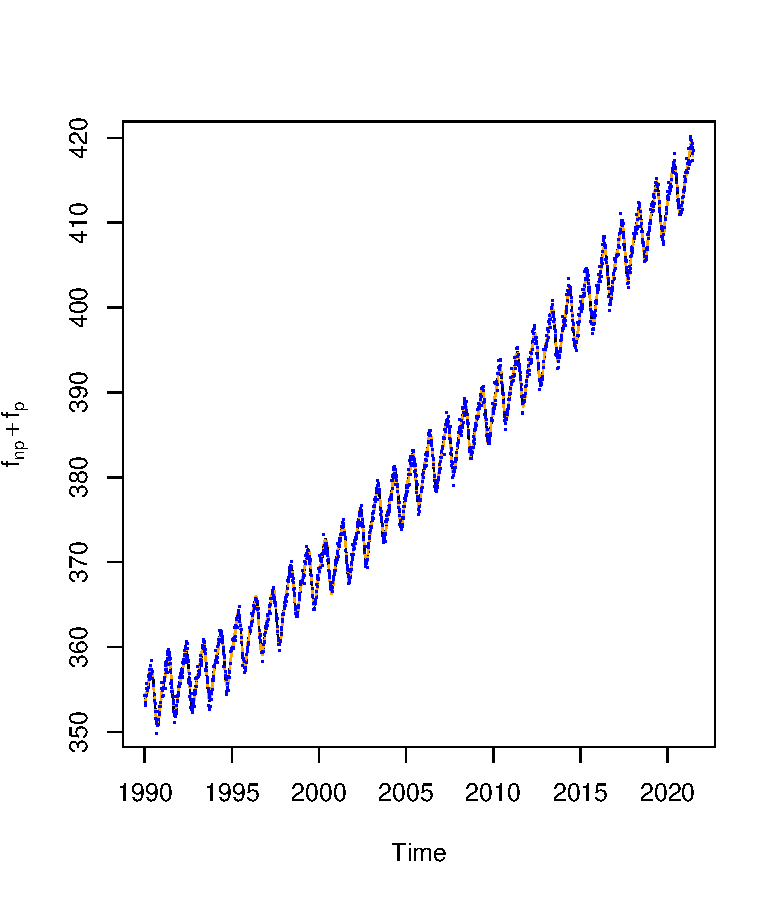
\includegraphics[width=0.45\textwidth]{1990_RW2_f.pdf}
    }
         \subfigure[Random effect $f_{np}$]{
      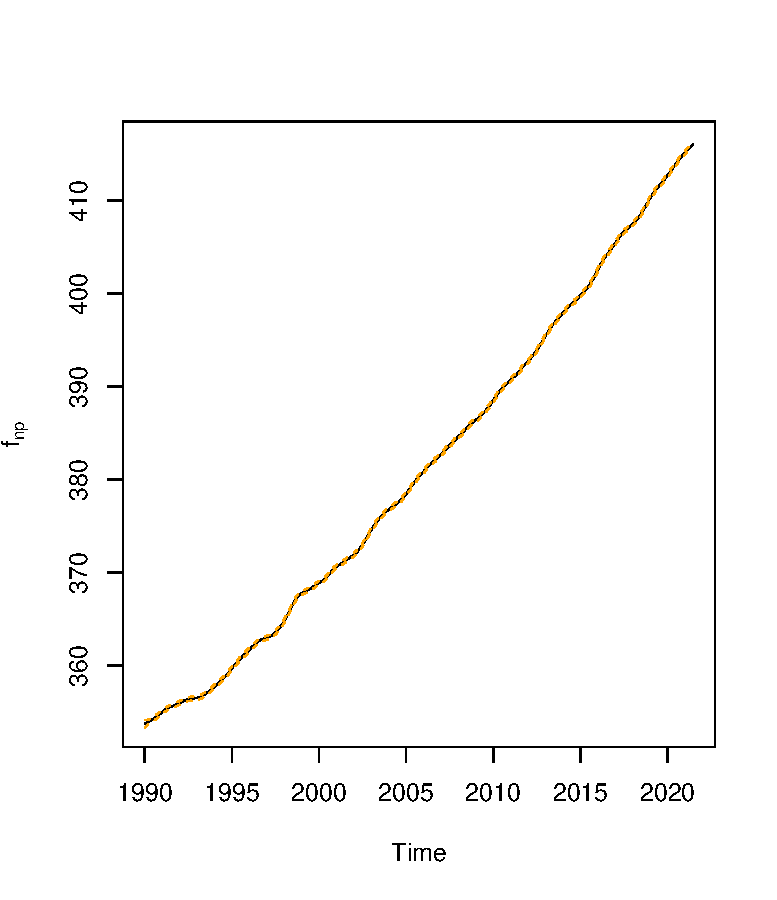
\includegraphics[width=0.45\textwidth]{1990_RW2_fnp.pdf}
    }
     \caption{Inference obtained for the CO2 dataset using RW2, for observations after year 1990.}
    \label{fig:realdata_1990}
\end{figure}
\end{frame}

\begin{frame}
\textbf{Looking at the variance and smoothing parameters:}
\begin{figure}[p]
    \centering
     \subfigure[Posterior for the smoothing parameter $\sigma_s$]{
      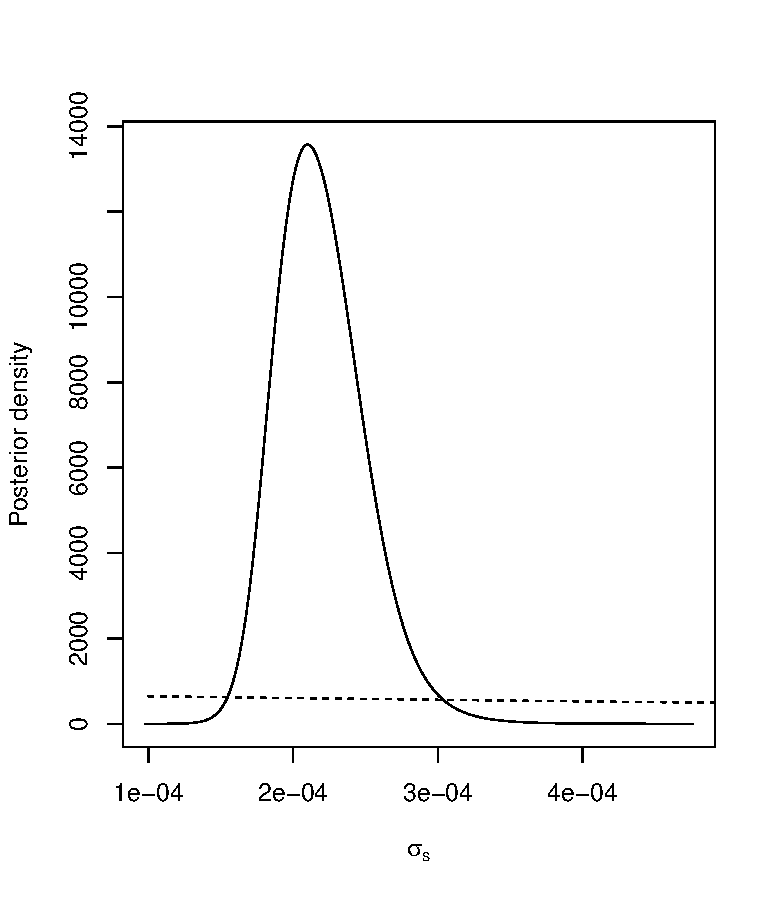
\includegraphics[width=0.39\textwidth]{1990_RW2_Hyper1.pdf}
    }
         \subfigure[Posterior for the variance parameter $\sigma_\epsilon$]{
      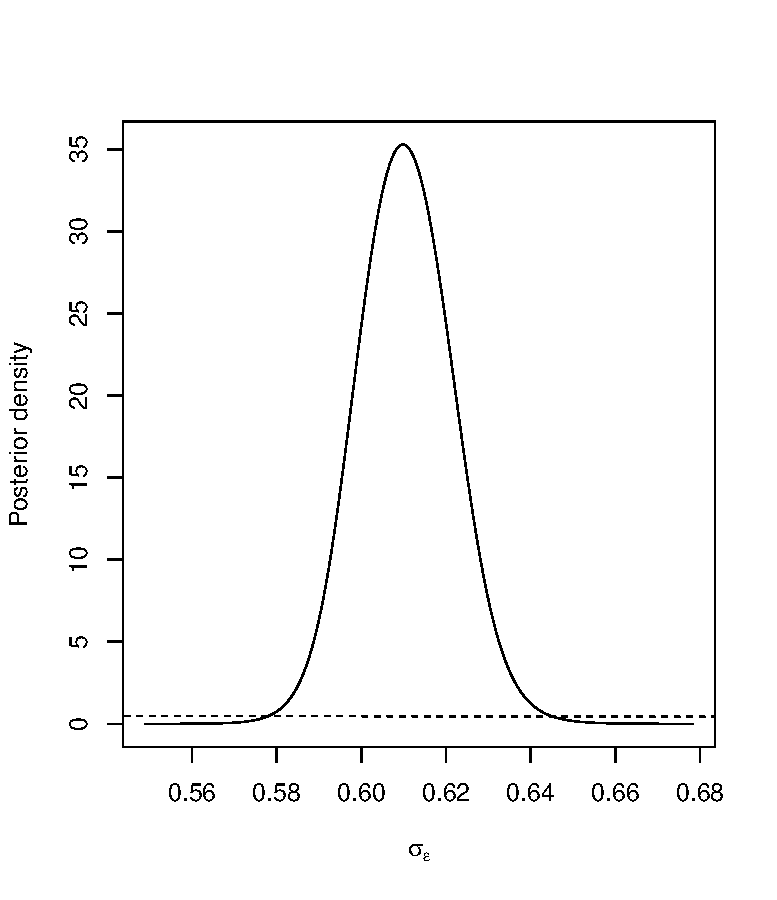
\includegraphics[width=0.39\textwidth]{1990_RW2_Hyper2.pdf}
    }
     \caption{Inference for smoothing/variance parameters with PC prior \citep{simpson2017penalising} with median 2.}
    \label{fig:realdata_1990_2}
\end{figure}
\end{frame}



\begin{frame}
\textbf{What about the derivatives?}

\begin{figure}[p]
    \centering
         \subfigure[$f'_{np}$ using RW2]{
      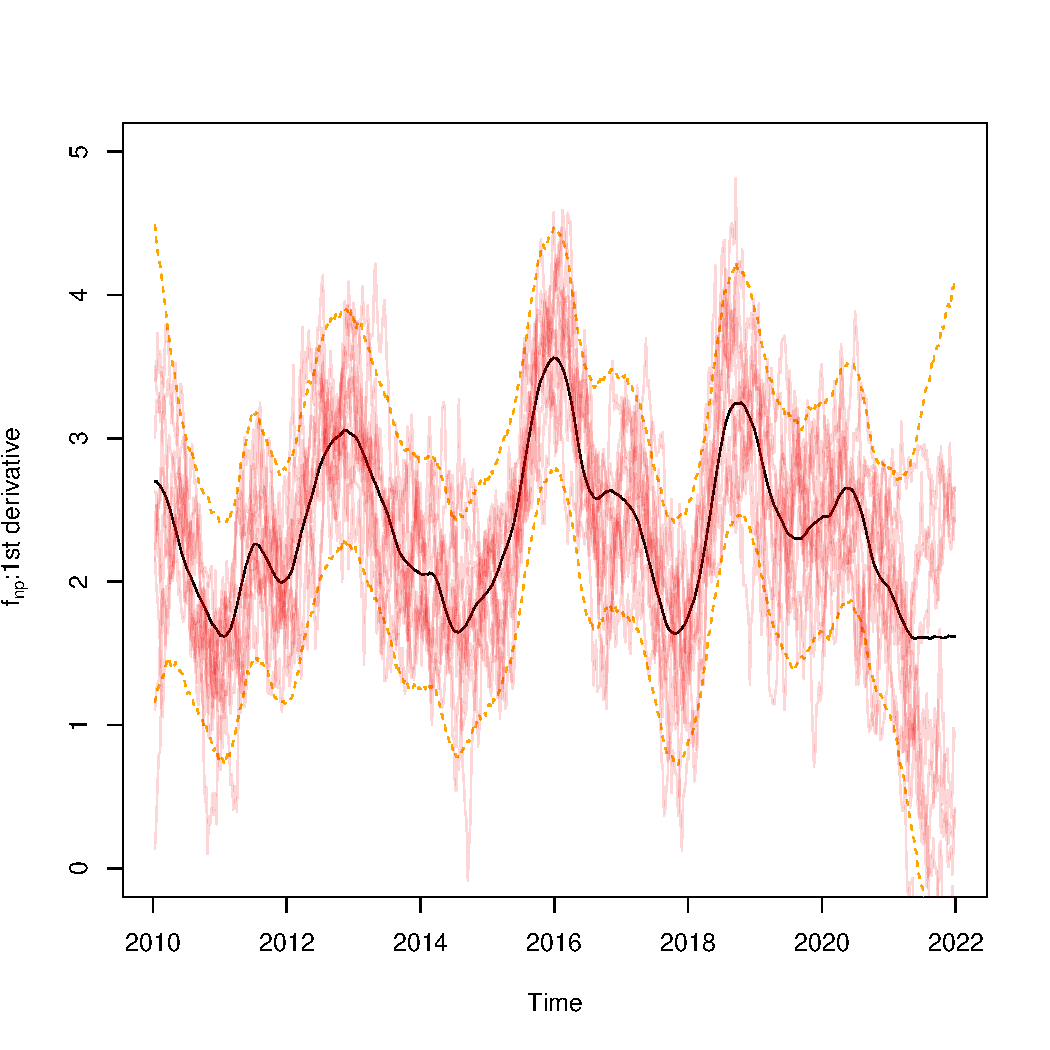
\includegraphics[width=0.45\textwidth]{2010_RW2_1st.pdf}
    }
         \subfigure[$f'_{np}$ using ARIMA]{
      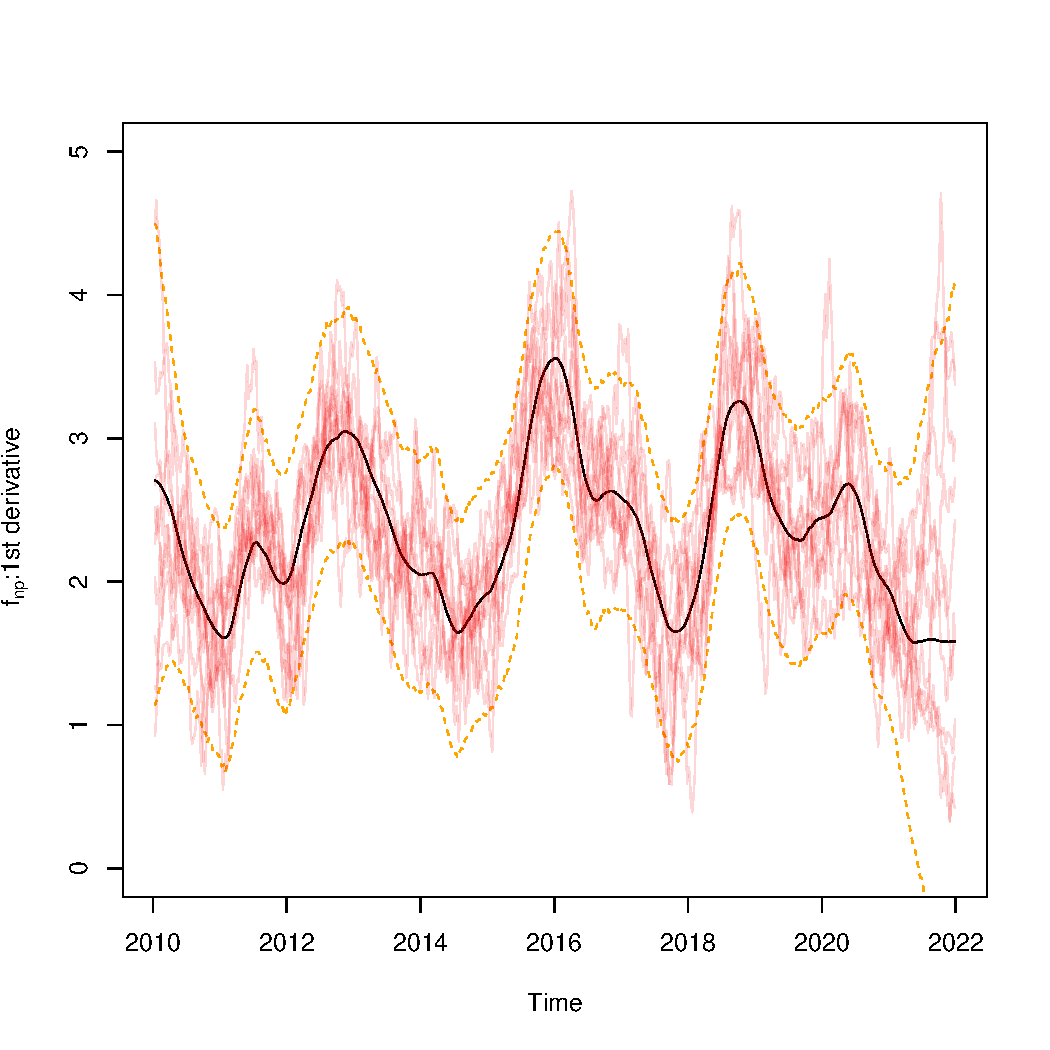
\includegraphics[width=0.45\textwidth]{2010_ARIMA_1st.pdf}
    }

    \label{fig:sim1-1replic}
\end{figure}
\end{frame}





\subsection{Simulation Study}

\begin{frame}
\textbf{A Simulation Study with 1000 independent replications:}

\begin{figure}[p]
    \centering
    \subfigure[MCI for $g'$]{
      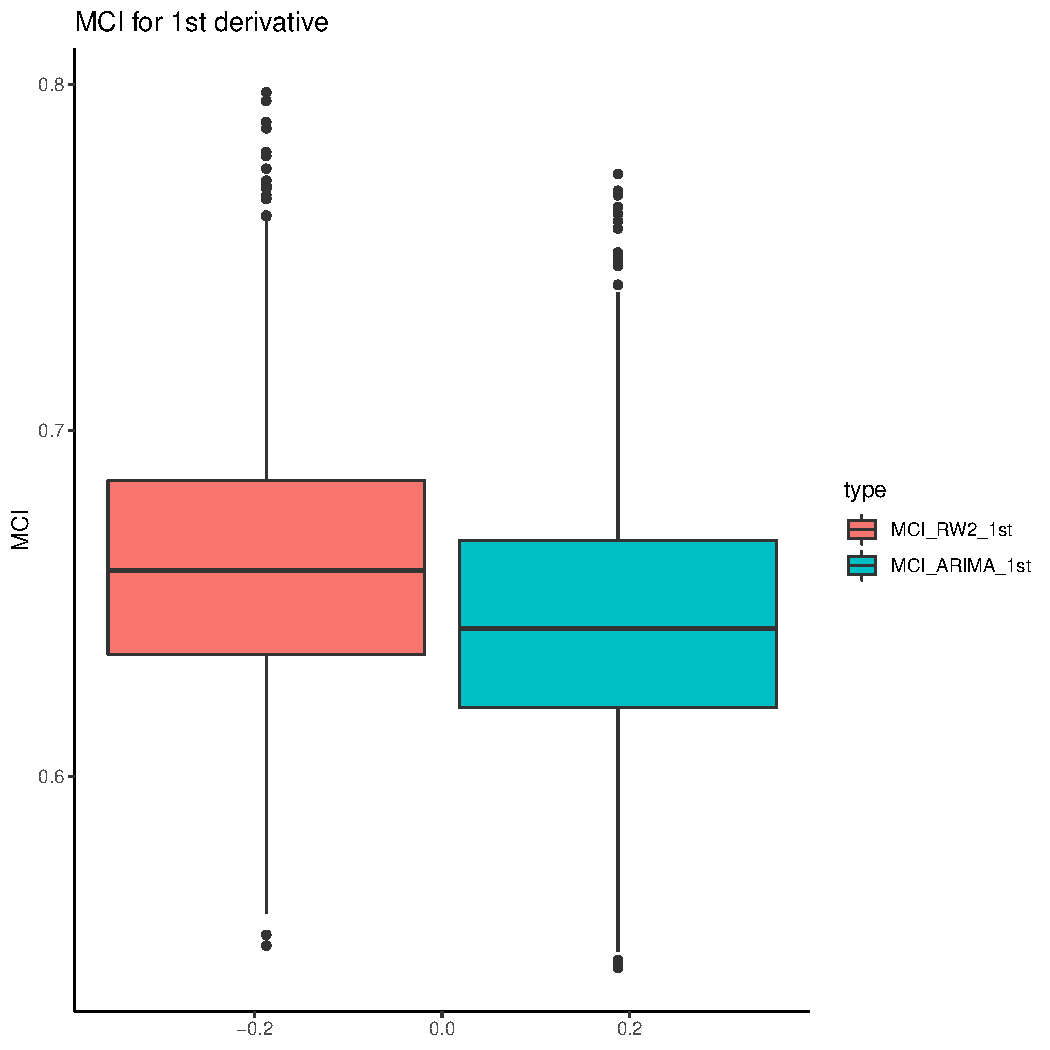
\includegraphics[width=0.45\textwidth]{sim1-g1st-MCI.pdf}
    }
     \subfigure[MCI for $g''$]{
      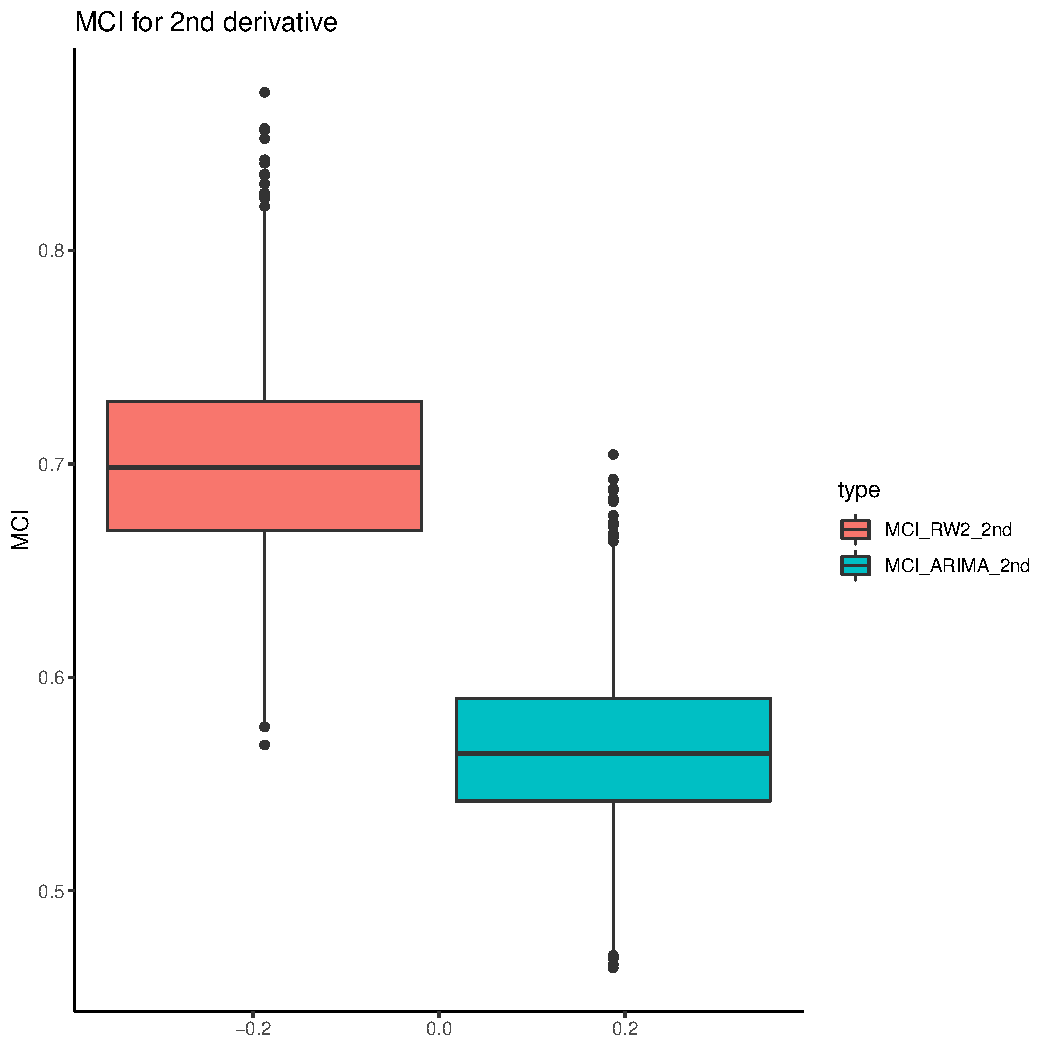
\includegraphics[width=0.45\textwidth]{sim1-g2nd-MCI.pdf}
    }
    \caption{Mean width of 90 percent credible interval (MCI) for $g',g''$ using RW2 or ARIMA, replicated for 1000 independent data sets.}
    \label{fig:sim1-1000replic}
\end{figure}
\end{frame}




\section{Conclusion and Next Step}

\begin{frame}
\begin{itemize}

\item We provide an overview of the extended second order random walk method \citep{rw2}, as well as its connection with the smoothing spline \citep{wahba} and the ARIMA prior \citep{ARIMA}.

\pause

\item The RW2 method gives similar result in terms of inference for $g$ as the ARIMA method, but less smooth inference for higher order derivatives of $g$ compared to ARIMA method.

\pause


\pause

\item We illustrate that It is possible to implement the exact ARIMA method with dense precision matrix. But which method is better should depend on the question of interest.

\end{itemize}
\end{frame}









\bibliography{refs}
\bibliographystyle{chicago}


\end{document}